% AA-63
\chapter[Klasyfikacja algebr Liego]{Sprzężoność podalgebr toralnych i klasyfikacja półprostych algebr Liego}
\label{aa:ch:lie-classification}

W AA-62 skonstruowaliśmy półprostą algebrę Liego dla każdej macierzy Cartana typu skończonego. Pozostał problem niezależności macierzy od wyboru maksymalnej podalgebry toralnej. Rozwiążemy go, wykazując sprzężoność takich podalgebr przez automorfizmy zbudowane z wykładników derywacji wewnętrznych. Potrzebny będzie elementarny fakt o obrazie odwzorowania wielomianowego nad ciałem algebraicznie domkniętym.

\section{Otwarte podzbiory w obrazie odwzorowania wielomianowego}

\begin{definicja}
\label{aa:def:lie-zariski-principal}
Niech $K$ będzie ciałem algebraicznie domkniętym i $n\ge1$. Dla wielomianu $p\in K[X_1,\ldots,X_n]$ piszemy
$D(p)=\{x\in K^n:p(x)\ne0\}$. Zbiory otwarte w topologii Zariskiego na $K^n$ są sumami mnogościowymi takich zbiorów.
\end{definicja}

Jeżeli $p,q$ są niezerowymi wielomianami, to $D(p)\cap D(q)=D(pq)\ne\varnothing$. Istotnie, pierścień wielomianów nad ciałem jest bez dzielników zera, a niezerowy wielomian nad nieskończonym ciałem nie znika na całym $K^n$ (indukcja po liczbie zmiennych). Nie potrzebujemy tu topologii euklidesowej.

\begin{lemat}[Obraz zawiera zbiór otwarty]
\label{aa:lem:lie-dominant-image}
Niech $K$ będzie algebraicznie domkniętym ciałem charakterystyki zero, $n\ge1$, $F=(F_1,\ldots,F_n):K^n\to K^n$ odwzorowaniem wielomianowym i $g\in K[X_1,\ldots,X_n]$ niezerowym wielomianem. Jeśli wyznacznik macierzy Jacobiego $F$ nie jest wielomianem zerowym, to istnieje niezerowy wielomian $p\in K[Y_1,\ldots,Y_n]$ taki, że
\[
 D(p)\subset F(D(g)).
\]
\end{lemat}
\begin{proof}
Oznaczmy $R=K[X_1,\ldots,X_n]$, $S=K[F_1,\ldots,F_n]\subset R$. Najpierw wykażemy, że $F_1,\ldots,F_n$ są algebraicznie niezależne. Gdyby istniał niezerowy wielomian $P$ z $P(F)=0$, wybierzmy taki o najmniejszym stopniu całkowitym. Różniczkując względem każdej zmiennej $X_j$, otrzymujemy
\[
 \sum_i (\partial_iP)(F)\,\partial_j F_i=0.
\]
Macierz Jacobiego jest odwracalna nad ciałem ułamków $R$, więc $(\partial_iP)(F)=0$ dla każdego $i$. Ponieważ $P$ nie jest stały i charakterystyka jest zero, co najmniej jedna pochodna jest niezerowym wielomianem mniejszego stopnia. Otrzymujemy sprzeczność. Zatem $S$ jest izomorficzny z $K[Y_1,\ldots,Y_n]$.

Ciało $L=K(X_1,\ldots,X_n)$ ma stopień przestępności $n$ nad $K$, a podciało $M=K(F_1,\ldots,F_n)$ również ma stopień przestępności $n$. Stąd $L/M$ jest algebraiczne: gdyby pewien element $L$ był przestępny nad $M$, wraz z $F_1,\ldots,F_n$ tworzyłby rodzinę $n+1$ elementów algebraicznie niezależnych nad $K$. Rozszerzenie $L/M$ jest skończone, ponieważ $L=M(X_1,\ldots,X_n)$ jest skończenie generowanym rozszerzeniem algebraicznym. Każdy z elementów $X_i$ i $g^{-1}$ spełnia więc równanie moniczne o współczynnikach w $M$. Wybierzmy niezerowy $d\in S$ będący iloczynem mianowników tych współczynników. W pierścieniu $A=S[d^{-1}]$ wszystkie te współczynniki już należą do $A$. Wobec tego
\[
 B=A[X_1,\ldots,X_n,g^{-1}]=R[d^{-1},g^{-1}]
\]
jest skończenie generowanym modułem nad $A$: dla każdego z dołączanych elementów równanie moniczne pozwala zastąpić każdą dostatecznie wysoką potęgę kombinacją niższych potęg. Iloczyny odpowiednio ograniczonych potęg wszystkich generatorów rozpinają $B$ nad $A$. Pierścienie $A,B$ są podpierścieniami $L$ i $A\subset B$.

Niech $p\in K[Y_1,\ldots,Y_n]$ odpowiada elementowi $d$ przez izomorfizm $Y_i\mapsto F_i$. Ustalmy $y\in D(p)$. Ewaluacja $F_i\mapsto y_i$ przedłuża się do surjekcji $A\to K$, której jądro $\mathfrak m$ jest ideałem maksymalnym. Pokażemy, że $\mathfrak mB\ne B$. Gdyby zachodziła równość, dla skończonego układu generatorów modułu $b_1,\ldots,b_s$ mielibyśmy
$b_i=\sum_j c_{ij}b_j$ z $c_{ij}\in\mathfrak m$. Po pomnożeniu układu $(I-C)b=0$ przez macierz dołączoną otrzymujemy $\det(I-C)b_i=0$ dla wszystkich $i$. Ponieważ generatory rozpinają również $1\in B$, mamy $\det(I-C)=0$ w $B$, a więc w $A$. Tymczasem modulo $\mathfrak m$ wyznacznik jest równy $1$. Sprzeczność.

Pierścień $B/\mathfrak mB$ jest więc niezerową skończenie wymiarową algebrą przemienną z jedynką nad $K$. Ma ideał maksymalny (można wybrać właściwy ideał największego wymiaru). Iloraz przez ten ideał jest skończonym rozszerzeniem ciała $K$, a ponieważ $K$ jest algebraicznie domknięte, jest równy $K$. Uzyskujemy homomorfizm $\psi:B\to K$ przedłużający ewaluację w $y$. Połóżmy $x_i=\psi(X_i)$. Ponieważ $\psi(g)\psi(g^{-1})=1$, mamy $x\in D(g)$. Ponadto $F_i(x)=\psi(F_i)=y_i$ dla wszystkich $i$. Tak więc $y\in F(D(g))$, co kończy dowód.
\end{proof}

\begin{przyklad}
\label{aa:prz:lie-dominant-image}
Odwzorowanie $F:K^2\to K^2$, $F(x,y)=(x,xy)$, ma wyznacznik Jacobiego równy $x$. Obraz zawiera $D(Y_1)$, lecz nie zawiera punktów $(0,b)$ dla $b\ne0$. Nie można zatem w Lemacie~\ref{aa:lem:lie-dominant-image} zastąpić tezy o niepustym zbiorze otwartym surjektywnością. Jeśli dodatkowo ograniczymy dziedzinę do $D(y)$, otrzymujemy dokładnie zbiór $\{(a,b):a\ne0,\ b\ne0\}$ wraz z punktem $(0,0)$.
\end{przyklad}

\section{Elementy regularne i automorfizmy wewnętrzne}

\begin{definicja}
\label{aa:def:lie-toral-regular}
Niech $\mathfrak g$ będzie niezerową skończenie wymiarową półprostą algebrą Liego nad algebraicznie domkniętym ciałem $K$ charakterystyki zero, $\mathfrak h$ jej maksymalną podalgebrą toralną i $\Phi$ zbiorem korzeni względem $\mathfrak h$. Element $t\in\mathfrak h$ nazywamy regularnym w $\mathfrak h$, jeśli $\alpha(t)\ne0$ dla każdego $\alpha\in\Phi$. Zbiór takich elementów oznaczamy przez $\mathfrak h_{\mathrm{reg}}$.
\end{definicja}

\begin{lemat}
\label{aa:lem:lie-regular-centralizer}
Przy założeniach Definicji~\ref{aa:def:lie-toral-regular} zbiór $\mathfrak h_{\mathrm{reg}}$ jest niepusty, a dla $t\in\mathfrak h$ zachodzi
\[
 Z_{\mathfrak g}(t)=\mathfrak h
 \quad\Longleftrightarrow\quad
 t\in\mathfrak h_{\mathrm{reg}},
\]
gdzie $Z_{\mathfrak g}(t)=\{x\in\mathfrak g:[t,x]=0\}$.
\end{lemat}
\begin{proof}
Iloczyn niezerowych funkcjonałów $\alpha$ jest niezerowym wielomianem na $\mathfrak h$, więc jego zbiór niezerowania jest niepusty. Z Twierdzenia~\ref{aa:tw:maximal-toral-cartan} mamy rozkład $\mathfrak g=\mathfrak h\oplus\bigoplus_{\alpha\in\Phi}\mathfrak g_\alpha$. Na $\mathfrak h$ operator $\operatorname{ad}_t$ znika, a na $\mathfrak g_\alpha$ jest mnożeniem przez $\alpha(t)$. Jego jądro to suma prosta $\mathfrak h$ i przestrzeni $\mathfrak g_\alpha$ dla tych korzeni, które znikają na $t$. Każda przestrzeń korzeniowa jest niezerowa, więc równoważność wynika wprost.
\end{proof}

\begin{definicja}
\label{aa:def:lie-elementary-inner}
Niech $\mathfrak g$ będzie skończenie wymiarową algebrą Liego nad ciałem $K$ charakterystyki zero. Przez $G_{\mathrm{el}}(\mathfrak g)$ oznaczamy podgrupę $\operatorname{Aut}_K(\mathfrak g)$ generowaną przez automorfizmy $\exp(\operatorname{ad}_x)$ dla wszystkich $x\in\mathfrak g$, dla których $\operatorname{ad}_x$ jest nilpotentny. Wykładnik jest skończoną sumą potęg operatora. Nie zakładamy tu istnienia grupy Liego ani struktury grupy algebraicznej na $G_{\mathrm{el}}(\mathfrak g)$.
\end{definicja}

To, że wykładniki są automorfizmami, wynika ze wzoru dwumianowego dla derywacji i z faktu, że ich odwrotnościami są wykładniki przeciwnych derywacji, jak w Lemacie~\ref{aa:lem:serre-reflections}. Dla każdego wektora korzeniowego $x\in\mathfrak g_\alpha$ operator $\operatorname{ad}_x$ jest nilpotentny: przenosi przestrzeń wagi $\lambda$ do przestrzeni wagi $\lambda+\alpha$. Ponieważ jest skończenie wiele wag, a w charakterystyce zero wagi $\lambda+k\alpha$ są parami różne, dostatecznie wysoka potęga tego operatora zeruje wszystkie składowe rozkładu.

\section{Sprzężoność maksymalnych podalgebr toralnych}

\begin{twierdzenie}
\label{aa:tw:lie-conjugate-toral}
Niech $\mathfrak g$ będzie niezerową skończenie wymiarową półprostą algebrą Liego nad algebraicznie domkniętym ciałem $K$ charakterystyki zero, a $\mathfrak h_1,\mathfrak h_2$ jej maksymalnymi podalgebrami toralnymi. Istnieje $\varphi\in G_{\mathrm{el}}(\mathfrak g)$ taka, że $\varphi(\mathfrak h_1)=\mathfrak h_2$.
\end{twierdzenie}
\begin{proof}
Ustalmy najpierw jedną maksymalną podalgebrę toralną $\mathfrak h$, jej zbiór korzeni $\Phi=\{\alpha_1,\ldots,\alpha_m\}$ i niezerowe wektory $x_j\in\mathfrak g_{\alpha_j}$. Indeksy oznaczają tu wszystkie korzenie, nie tylko proste. Przez $r$ oznaczmy wymiar $\mathfrak h$. Przestrzenie korzeniowe są jednowymiarowe na mocy wyników AA-60, zatem $\dim\mathfrak g=m+r$. Rozważmy odwzorowanie
\[
\begin{split}
 F_{\mathfrak h}:K^m\times\mathfrak h&\longrightarrow\mathfrak g,\\
 (s,t)&\longmapsto
 \exp(s_1\operatorname{ad}_{x_1})\cdots
 \exp(s_m\operatorname{ad}_{x_m})t.
\end{split}
\]
Jest wielomianowe, ponieważ wszystkie wykładniki są skończonymi sumami. Dla $t_0\in\mathfrak h_{\mathrm{reg}}$ jego różniczka w $(0,t_0)$ jest równa
\[
 (\xi,v)\longmapsto
 v+\sum_{j=1}^m \xi_j[x_j,t_0]
 =v-\sum_{j=1}^m\xi_j\alpha_j(t_0)x_j.
\]
Istotnie, współczynnik liniowy względem $s_j$ w wykładniku to $\operatorname{ad}_{x_j}$, a pozostałe wykładniki w zerze są identycznością. Różniczka jest izomorfizmem na mocy rozkładu korzeniowego i niezerowości wszystkich $\alpha_j(t_0)$.

Po wyborze baz dziedzina i przeciwdziedzina mają postać $K^{m+r}$. Warunek $t\in\mathfrak h_{\mathrm{reg}}$ jest niezerowaniem wielomianu $g(s,t)=\prod_{\alpha\in\Phi}\alpha(t)$. Z Lematu~\ref{aa:lem:lie-dominant-image} otrzymujemy niepusty zbiór $D(p_{\mathfrak h})\subset\mathfrak g$ zawarty w obrazie $K^m\times\mathfrak h_{\mathrm{reg}}$. Każdy element tego zbioru jest obrazem pewnego regularnego elementu $\mathfrak h$ przez automorfizm należący do $G_{\mathrm{el}}(\mathfrak g)$.

Wykonujemy konstrukcję dla $\mathfrak h_1$ i $\mathfrak h_2$, używając tej samej bazy przeciwdziedziny $\mathfrak g$. Zbiory $D(p_{\mathfrak h_1})$ i $D(p_{\mathfrak h_2})$ przecinają się, gdyż iloczyn dwóch niezerowych wielomianów nie jest zerowy. Wybierzmy $z$ w ich przecięciu. Istnieją $t_i\in(\mathfrak h_i)_{\mathrm{reg}}$ oraz $\psi_i\in G_{\mathrm{el}}(\mathfrak g)$ takie, że $z=\psi_i(t_i)$ dla $i=1,2$. Automorfizm Liego przenosi centralizator elementu na centralizator jego obrazu, więc
\[
 Z_{\mathfrak g}(z)
 =\psi_1(\mathfrak h_1)=\psi_2(\mathfrak h_2)
\]
na mocy Lematu~\ref{aa:lem:lie-regular-centralizer}. Wystarczy przyjąć $\varphi=\psi_2^{-1}\psi_1$.
\end{proof}

\begin{center}
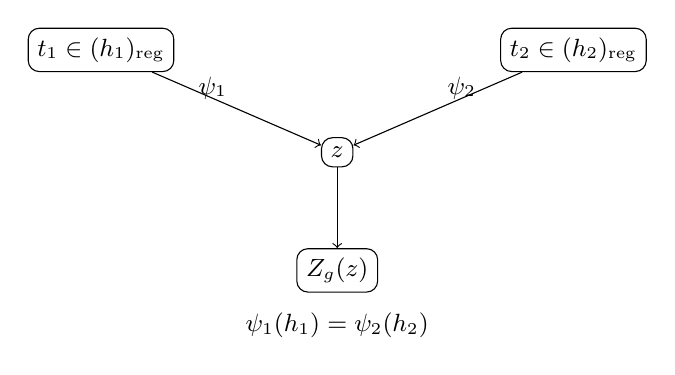
\begin{tikzpicture}[every node/.style={font=\small}]
\node[draw,rounded corners] (a) at (-3,1.3) {$t_1\in(\mathfrak h_1)_{\mathrm{reg}}$};
\node[draw,rounded corners] (b) at (3,1.3) {$t_2\in(\mathfrak h_2)_{\mathrm{reg}}$};
\node[draw,rounded corners] (z) at (0,0) {$z$};
\node[draw,rounded corners] (h) at (0,-1.5) {$Z_{\mathfrak g}(z)$};
\draw[->] (a)--node[above left] {$\psi_1$} (z);
\draw[->] (b)--node[above right] {$\psi_2$} (z);
\draw[->] (z)--(h);
\node at (0,-2.2) {$\psi_1(\mathfrak h_1)=\psi_2(\mathfrak h_2)$};
\end{tikzpicture}

\small Wspólny obraz elementów regularnych prowadzi do równości centralizatorów.
\end{center}

\begin{wniosek}
\label{aa:cor:lie-rank-invariant}
Wszystkie maksymalne podalgebry toralne niezerowej skończenie wymiarowej półprostej algebry Liego nad algebraicznie domkniętym ciałem charakterystyki zero mają ten sam wymiar. Nazywamy go rzędem algebry Liego. Macierz Cartana, z dokładnością do jednoczesnej permutacji wierszy i kolumn, nie zależy od wyboru maksymalnej podalgebry toralnej ani bazy układu korzeni.
\end{wniosek}
\begin{proof}
Pierwsza teza wynika z istnienia izomorfizmu podalgebr w Twierdzeniu~\ref{aa:tw:lie-conjugate-toral}. Jeżeli $\varphi(\mathfrak h_1)=\mathfrak h_2$, to dla $x\in\mathfrak g_\alpha$ i $t\in\mathfrak h_1$ zachodzi $[\varphi(t),\varphi(x)]=\alpha(t)\varphi(x)$. Zatem $\alpha\mapsto\alpha\circ\varphi^{-1}$ przenosi zbiór korzeni względem $\mathfrak h_1$ bijektywnie na zbiór względem $\mathfrak h_2$. Automorfizm zachowuje formę Killinga, więc przenosi $t_\alpha$ z AA-59 na $t_{\alpha\circ\varphi^{-1}}$ oraz $h_\alpha$ na odpowiadający element drugiej podalgebry. W szczególności zachowuje wszystkie liczby Cartana. Przeniesienie układu zachowuje też całkowite zależności w bazie, więc przenosi bazę na bazę. Dowolne dwie bazy tego samego układu różnią się działaniem grupy Weyla jako zbiory, na mocy Twierdzenia~\ref{aa:tw:weyl-chambers}. Odbicia zachowują liczby Cartana; ewentualna zmiana numeracji powoduje jednoczesną permutację wierszy i kolumn.
\end{proof}

\begin{przyklad}[Elementy regularne w $\mathfrak{sl}_2(K)$]
\label{aa:prz:lie-regular-sl2}
Niech $K$ będzie algebraicznie domkniętym ciałem charakterystyki zero. W $\mathfrak{sl}_2(K)$ przyjmijmy $h=\operatorname{diag}(1,-1)$, $e=E_{12}$, $f=E_{21}$ i $\mathfrak h=Kh$. Dla $t=ch$ korzenie przyjmują wartości $2c$ i $-2c$. Zatem $t$ jest regularny w $\mathfrak h$ dokładnie wtedy, gdy $c\ne0$. Dla $x=ah+be+df$ mamy $[t,x]=2cbe-2cdf$, więc dla $c\ne0$ centralizatorem jest $Kh$, a dla $c=0$ cała algebra.

Wybierzmy kolejność korzeni $e,f$. Ponieważ $e^2=f^2=0$ jako macierze, $\exp(s\operatorname{ad}_e)$ i $\exp(u\operatorname{ad}_f)$ są sprzężeniami przez $I+se$ i $I+uf$: po rozwinięciu iloczynu $(I+se)x(I-se)$ otrzymujemy $x+s[e,x]-s^2exe$, a $[e,[e,x]]=-2exe$ i trzecia potęga derywacji znika. Dla $f$ rachunek jest identyczny. Różniczka odwzorowania $F_{\mathfrak h}$ w punkcie $(0,0,ch)$ ma w bazie $(e,f,h)$ postać
\[
 (\xi,\eta,v)\longmapsto -2c\xi e+2c\eta f+vh.
\]
Jej wyznacznik wynosi $-4c^2$, a więc jest niezerowy dokładnie dla elementów regularnych. Widać bezpośrednio, dlaczego w dowodzie sprzężoności nie wystarcza dowolny element podalgebry toralnej.
\end{przyklad}

\section{Klasyfikacja algebr prostych i półprostych}

\begin{twierdzenie}[Klasyfikacja]
\label{aa:tw:lie-semisimple-classification}
Niech $K$ będzie algebraicznie domkniętym ciałem charakterystyki zero. Klasy izomorfizmu niezerowych skończenie wymiarowych prostych algebr Liego nad $K$ (prostych w sensie nieabelowym) są w bijekcji z typami nierozkładalnych skończonych diagramów Dynkina
\[
 A_n\ (n\ge1),\quad B_n\ (n\ge2),\quad
 C_n\ (n\ge3),\quad D_n\ (n\ge4),
\]
oraz $E_6,E_7,E_8,F_4,G_2$. Typ $C_2$ opisuje tę samą klasę co $B_2$. Klasy wszystkich skończenie wymiarowych półprostych algebr Liego odpowiadają skończonym wielozbiorom tych typów, przy czym pusty wielozbiór odpowiada algebrze zerowej.
\end{twierdzenie}
\begin{proof}
Niezerowa algebra prosta jest półprosta, ponieważ jej jedynymi ideałami są zero i ona sama, a nieabelowa algebra prosta jest równa własnej algebrze pochodnej. Dla półprostej algebry wybieramy maksymalną podalgebrę toralną i bazę układu korzeni. Otrzymana macierz Cartana jest typu skończonego, na mocy AA-60 i Twierdzenia~\ref{aa:tw:root-cartan}. Z Twierdzenia~\ref{aa:tw:lie-dynkin-components} algebra jest prosta wtedy i tylko wtedy, gdy diagram jest spójny.

Dla każdego typu z listy istnieje układ korzeni realizujący odpowiednią macierz Cartana (Wniosek~\ref{aa:cor:root-classification} wraz z konstrukcjami poprzedzającymi go). Twierdzenie~\ref{aa:tw:serre-existence} konstruuje półprostą algebrę Liego dla tego układu. Jeżeli diagram jest spójny, algebra jest prosta. Dwie algebry o tej samej macierzy są izomorficzne na mocy Twierdzenia~\ref{aa:tw:serre-presentation}. Odwrotnie, izomorfizm algebr przenosi maksymalną podalgebrę toralną na maksymalną podalgebrę toralną (zachowuje abelowość i diagonalizowalność reprezentacji dołączonej). Przenosi też przestrzenie korzeniowe i formę Killinga. Wniosek~\ref{aa:cor:lie-rank-invariant} pokazuje, że macierze Cartana obu algebr różnią się co najwyżej permutacją indeksów. Twierdzenie~\ref{aa:tw:finite-dynkin} daje dokładnie podaną listę, z usuniętym powtórzeniem $C_2$.

W przypadku dowolnej niezerowej algebry półprostej stosujemy Twierdzenie~\ref{aa:tw:lie-dynkin-components}: każda składowa spójna wyznacza prosty ideał, a algebra jest ich sumą prostą. Odwrotnie, suma prosta skończonej rodziny prostych algebr jest półprosta, gdyż obraz rozwiązalnego ideału przez każdą projekcję byłby rozwiązalnym ideałem odpowiedniej prostej algebry, czyli zerem. Suma wybranych maksymalnych podalgebr toralnych w składnikach jest toralna i równa swojemu centralizatorowi (centralizator liczymy osobno w każdym składniku). Jest zatem maksymalna toralna, a jej układ korzeni jest rozłączną sumą układów składników. Macierz Cartana jest blokowo diagonalna. Dwie takie sumy są izomorficzne wtedy i tylko wtedy, gdy ich macierze są równoważne przez jednoczesną permutację indeksów, czyli gdy mają identyczny wielozbiór typów składowych spójnych. Przypadek algebry zerowej nie wymaga wyboru korzeni.
\end{proof}

\begin{przyklad}[Dlaczego wymiar i rząd nie wystarczają]
\label{aa:prz:lie-bc-classification}
Dla $n\ge3$ typy $B_n$ i $C_n$ mają po $2n^2$ korzeni: w modelu $B_n$ występują $\pm e_i$ i $\pm e_i\pm e_j$ ($i<j$), a w $C_n$ zamiast $\pm e_i$ występują $\pm2e_i$. Obie algebry mają zatem wymiar $n+2n^2$ i rząd $n$. Nie są jednak izomorficzne. Ich diagramy mają przeciwnie skierowaną podwójną krawędź, a dla $n\ge3$ jej dwa końce mają różne stopnie w grafie. Nie istnieje więc permutacja zachowująca graf i zamieniająca te końce. Macierze Cartana nie są równoważne, a Twierdzenie~\ref{aa:tw:lie-semisimple-classification} wyklucza izomorfizm. Dla $n=2$ oba końce mają stopień jeden, więc zamiana indeksów rzeczywiście utożsamia typy.
\end{przyklad}

\begin{uwaga}
Udowodniliśmy sprzężoność maksymalnych podalgebr toralnych, które są podalgebrami Cartana na mocy AA-59. Nie dowodziliśmy tu osobno, że każda nilpotentna podalgebra równa swojemu normalizatorowi jest maksymalną podalgebrą toralną. Taka równoważność nie jest potrzebna do powyższej klasyfikacji.
\end{uwaga}
